\chapter{関連研究}
この章ではまず、既存のボードゲームAIについてAlphaZeroを中心に強化学習的枠組みからその理論を説明する。
次にAlpha Zeroの問題点とそれを補完する既存手法とその課題について述べる。



\section{強化学習\cite{RL}}
強化学習はタスクを選択をする主体と環境のやり取りとして定式化し、その相互作用から学習する形でタスクに取り組む分野である。
状態$s$と行動$a$が次の状態${s'}(=T(s, a), Tは遷移関数)$と環境から与えられる報酬$r$が決定されると仮定する。その仮定の下、環境から与えられる報酬の合計$G$(以下収益と記載)を最大化する。
報酬を大きくするためには状態sに応じて適切な(より大きな報酬をもらえる可能性が高い)行動を選択する必要がある。
ある状態$s$である行動$a$をとった場合の収益に対して見積もりをとり、見込まれる値が最も大きい行動を選択することでより大きな収益を獲得できると期待できる。
このようなある状態である行動を取った場合の収益の見積もりを$Q(s, a)$とした場合、
\begin{equation}
	{\displaystyle a_m = {\textrm{argmax}}_{a} Q(s, a)}
\end{equation}
となる$a_m$を選択することによって収益の最大化が期待される。また、ある状態から獲得できる収益の合計の予想値$V(s)$(以下状態価値関数と表記)は、最適な行動$a_m$を取った場合の値として推定される。
\begin{equation}
	{\displaystyle V(s) = Q(s, a_m)(a_m = \textrm{argmax}_{a} Q(s, a))}
\end{equation}
強化学習手法によってタスクの最適化を図る際にはこの$V(s),Q(s, a)$を正しく推定することが直接的な目標となる。$V(s),Q(s, a)$は主体が実際に環境とやり取りを行う(タスクを実行していく)中で改善されていき、
Temporary Difference法やMonte Carlo法等が基本的な$V(s),Q(s, a)$の更新則である。また、DQN\cite{DQN}やRainbow\cite{rainbow}等はニューラルネットワークを使用して$V(s),Q(s, a)$
を推定することでより高い性能を発揮している。



\subsection{ボードゲームへの応用}
ボードゲームでは通例、状態sは盤面の状況、行動はプレイヤーの選択、報酬はゲームの最後に勝敗として与えられる。
状態$s$(ゲームの状況)と行動$a$(プレイヤーの選択)によって盤面は次の状態$s'$に遷移し、次の行動$a'$(他のプレイヤーによる選択)を受け付ける、というサイクルにゲームの進行を定式化して表現することができる。
また、上述した強化学習における$V(s)$の推定は「ある盤面はプレイヤーにとって勝利に近いのか」を表現していると解釈される。
AlphaGo\cite{AlphaGo}やStockFish\cite{StockFish}、DeepLearningShogi\cite{dlshogi}では状態$s$は最新$N$ステップの盤面や手数などのゲームのプレイにおいて重要な情報である。
状態は行列等の形式に抽象化され、行動は次にプレイヤーが打つ箇所の座標となる。
\begin{figure}[t]
	\centering
	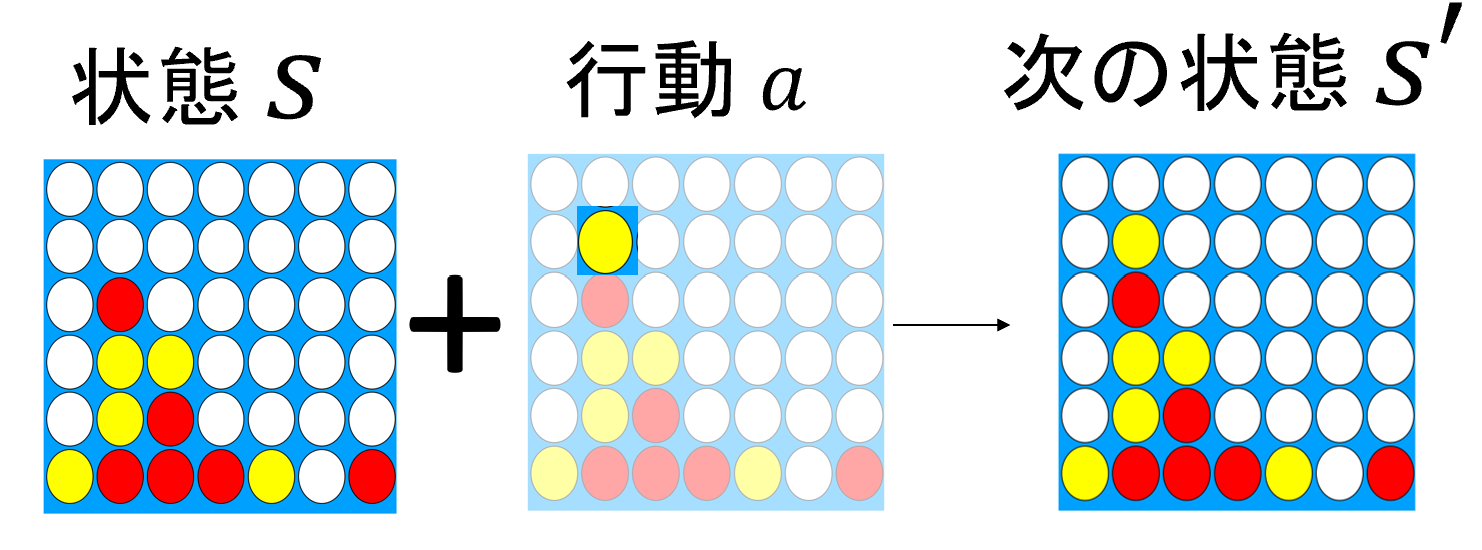
\includegraphics[width=\linewidth]{./figure/transition.png}
	\caption{ボードゲームにおける強化学習モデル}
	\label{fig:transition}
\end{figure}

本論文で使用したalphazero\_baselineにおける入力は最新の盤面の状態を空白を0, 先番(赤)の石の位置を1, 後ろ
番(黄)の位置を-1として抽象化した6$\times$7の行列となる。
また、後述するconnect4のルール上の制約により次にプレイヤーが打つ箇所(行動)は列の数と同数の7つに限定される。

\subsection{AlphaZero\cite{AlphaZero}}
AlphaZeroは2016年に登場し、元世界チャンピオンであるイ・セドルに対して四勝一敗の成績を収めたAlphaGoの汎用版である。
AlphaZeroは先述の$V(s),Q(s, a)$を推定する際にニューラルネットワークとPV-モンテカルロ木探索システムを使用する。
\paragraph{ニューラルネットワーク}
AlphaZero内のニューラルネットワークに対する入力は最新$8$ステップの盤面($\left\{ s_{-7}, ..., s_0 \right\}$,$s_{-i}$は$i$ステップ前の盤面,$s_{0}$は現在の盤面)であり、出力は方策$P(\left\{ s_{-7}, ..., s_0 \right\})$と
局面評価$V(\left\{ s_{-7}, ..., s_0 \right\})$の二種類である。\
ネットワークは1つの畳み込み層と20の残差結合ネットワークで構成されている。方策は「現在の状況$s_0$から次にどこを選択すべきか」を表現しており、次に選択すべき座標を確率分布の形式で表現する。
alphazero\_baselineにおける選択肢は列の数と等しい7であるため、1$\times$7の行列となる。方策内の値が大きさがAIによるその着手の評価と解釈され、成分が大きい座標を次に選択することが推奨される。例えば方策が
$\left\{0, 0.1, 0.2, 0, 0, 0.7, 0.8\right\}$であるとき、方策中の最も大きい成分は7番目の0.8であるため、プレイヤーは次に7列目を選択する事が推奨される。
また、局面評価$V(\left\{ s_{-7}, ..., s_0 \right\})$は「(過去8ステップ分の状態を含めた)現在の状況$s_0$は勝利に近いのか」を表現しており、値が上限に近ければ近い程、現在の状況$s_0$が次の着手を選択するプレイヤーにとっての勝利に近いことを表している。

訓練とかどうするん?
\begin{figure}[t]
	\centering
	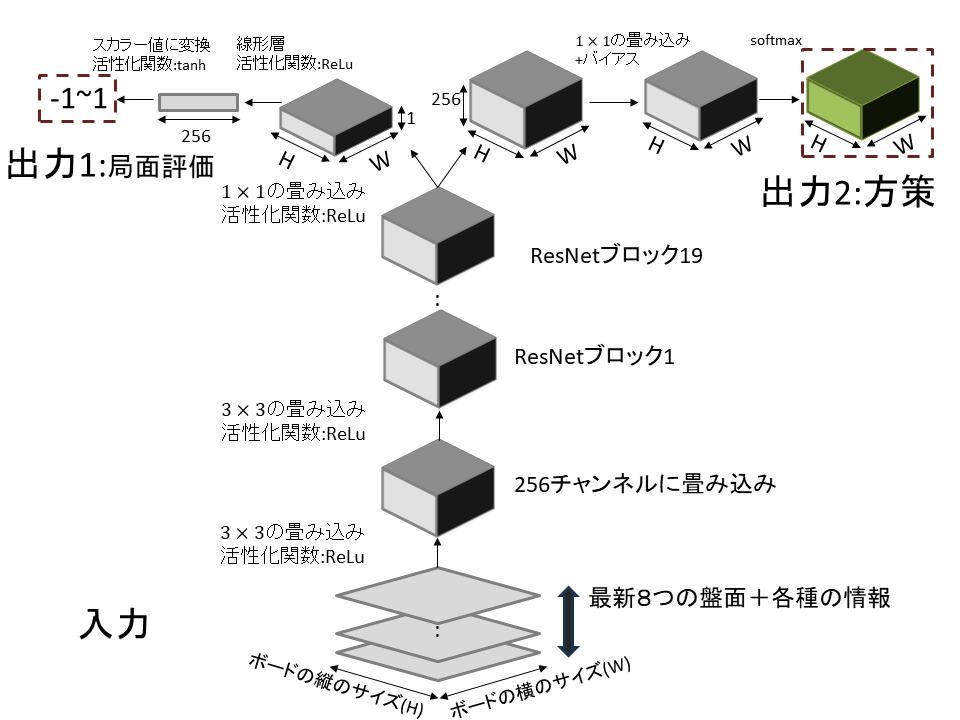
\includegraphics[width=\linewidth]{./figure/network.png}
	\caption{AlphaZeroネットワークのイメージ}
	\label{fig:network}
\end{figure}
\paragraph{PV-モンテカルロ木探索}
PV-モンテカルロ木探索ではニューラルネットワークから得た方策$P(s)(以下s=\left\{ s_{-N+1}, ..., s_0 \right\}と表記する)$と局面評価$V(s)$をシミュレーション
によって改善する。
PV-モンテカルロ木探索ではシミュレーションによって$s$をノード、各行動$a$を枝とした決定木を構築する。
最終的に各ノード$s$から派生する各行動$a$の分布$\left\{a_0, a_1, ..., a_n\right\}$が改善された方策となる。
一方、局面評価もまたモンテカルロ木探索により決定木が拡張されるなかで更新される。?ページに決定木と局面評価$V(s)$の詳細な更新アルゴリズムを示し、ここでは大まかな流れを示す。。
step1ではまず、探索の開始地点となるノード$s$を決定する。次にStep2:再帰部分では以下の処理を再起的に呼び出す。
\begin{enumerate}
	\item ノードを探索したことがない場合
	ニューラルネットワークから出力された方策$P(s)$と局面評価$V(s)$を返却する
	\item ノードを探索したことがある場合
	以下のpuctスコア$U(s, a)$に従い、子ノード$s_c$を選び、$s_c$に対して再帰的に探索を行いその結果である$P(s_e), V(s_e)(s_eは再帰処理の結果たどり着く
	決定木の端のノード)$を返却する。($N(s), N(s, a)はそれぞれs,(s, a)に対して探索を行った回数$)
	\begin{equation}
		{U(s, a)= C(s)P(s, a)\frac{\sqrt{N(s)}}{1+N(s, a)}\\
		}
	\end{equation}
	
	\begin{equation}
		{C(s)=\textrm{log}\frac{1+N(s)+C_{\textrm{base}}}{C_{\textrm{base}}}+C_{\textrm{init}}\\
		(C_{\textrm{base}}, C_{\textrm{init}}はハイパーパラメータ)}
	\end{equation}
\end{enumerate}
このようなプロセスによって構築された決定木を用いてモデルは対戦を行う。
\newpage
\begin{algorithm}
    \caption{PV-MCTS in AlphaZero (Part 1: Exploration)}
    \begin{algorithmic}[1]
        \State $t$: 決定木
        \State $T$: 遷移関数
        \State $N(s, a)$: $(s, a)$の組み合わせを探索した回数
        \State $Q(s, a)$: 行動価値関数 ($\textrm{Explore}(s)$の平均)
        \State $W(s, a)$: 行動価値の総和$(W(s, a)=Q(s, a)N(s, a))$
        \State $P(s, a)(=P(s_n), s_n=T(s, a))$: 
        \State ニューラルネットワークから出力された方策
        \State $V(s, a)(=V(s_n), s_n=T(s, a))$: 
        \State ニューラルネットワークから出力された局面評価
        \Function{Explore}{$s_{\text{start}}$}
            \State Set $s_{now} = s_{start}$ and $a_{now} = a_m$
            \For {each simulation}
                \State $\zeta \gets empty list$
                \State $s_{\text{current}} \gets s_{\text{start}}$
                \While {$s_{\text{current}}$ がゲームの終了状態でない場合}
                    \State $a_t \gets TreePolicy(s)$
                    \State (Tは遷移関数)
                    \State $(s_{\text{current}}, a_t)$を $\zeta $の末尾に追加
                    \State $s_{\text{next}} \gets T(s_{\text{current}}, a_t)$
                    \State $s_{\text{current}} \gets s_{\text{next}}$
                    
                \EndWhile
                \State $G \gets V(s_e)$ 
                \State($s_e$は$s_{start}$から探索してたどり着いたノード$s_e$)
                \State \Call{Backpropagate}{$\zeta, G$}
            \EndFor
        \EndFunction
        
        
    \end{algorithmic}
\end{algorithm}
\begin{algorithm}
    \caption{PV-MCTS in AlphaZero (Part 2: Backpropagation)}
    \begin{algorithmic}[1]
        \Function{TreePolicy}{$s$}
            \If {$s$が探索されていない子ノードを持つとき}
                \State $s_c \gets T(s, a)$ ($s_c$は未探索のノード)
                \State \Call{InitNode}{$s_c$}
                \State \Return $a$
            \Else
                \State 以下のPUCTスコア$U(s, a)$を計算
                \State $U(s, a)= C(s)P(s, a)\frac{\sqrt{N(s)}}{1+N(s, a)}$
                \State $C(s)=\textrm{log}\frac{1+N(s)+C_{\textrm{base}}}{C_{\textrm{base}}}+C_{\textrm{init}}$
                \State($C_{\textrm{base}}$, $C_{\textrm{init}}$はハイパーパラメータ)
                \State $(N(s)=\Gamma N(s, a))$
                \State 以下のように$a$を求める
                \State $a = {\textrm{argmax}}_a (Q(s, a)+U(s, a))$
                \State \Return $a$
                
            \EndIf
        \EndFunction
        \Function{Backpropagate}{$\zeta, G$}
            \For {each node-action pair $(s, a)$ in $\zeta$}
                \State $N(s, a) \gets 0$
                \State $W(s, a) \gets 0$
                \State $Q(s, a) \gets 0$
            \EndFor
        \EndFunction
        \Function{InitNode}{$s$}
            \For {each action $a$ from  $s$}
                \State $N(s, a) \gets N(s, a)+1$
                \State $W(s, a) \gets W(s, a)+G$
                \State $Q(s, a) \gets \frac{W(s, a)}{N(s, a)}$
            \EndFor
        \EndFunction
    \end{algorithmic}
\end{algorithm}


\subsection{ボードゲームAIの問題点}
StockFish\cite{StockFish}やDeepLearningShogi\cite{dlshogi}などの従来のボードゲームAIはそのゲーム固有の知識(ドメイン知識)に基づくものが多く、「ある条件を満たすときにある選択をする」と言ったようにその挙動をルールとして表すことが可能である。
一方でAlphaZeroのニューラルネットワークと木探索を組み合わせた手法では方策と局面評価の根拠を得ることができない、つまりAlphaZeroの問題点として説明性の欠如が挙げられるのである。
説明性の欠如はAIの判断に対する責任の不在を意味し、優れた性能を持つシステムのより、ハイレベル、ハイリスクなタスクへの実用化に対する障害となる。



\section{XAI}

\subsection{概要}
XAIとはexplainable AI(説明可能AI)の略語であり、AIを人間に対して説明可能なものにする、もしくは説明可能なAIを構築する領域である。
本論文はAIの判断根拠として先読みを示す意味でXAIの分野に属する研究であると言える。
ここでの「説明可能性」の語は「人間に理解できる形での説明を与える能力」\cite{definition}と定義され、
「いつ、どのような、どのように」説明を与えるかによってさらに細かく分類される。
「いつ」、つまりどの時点で説明を与えるか、に関しては既存のネットワークに対して新たに説明を加える「事後的」説明と初めから動作の根拠を示せるようにネットワークやシステムを構築する「事前的」説明
に分類できる\cite{definition}。
「どのような」、つまり説明の内容については「大域的」説明と「局所的」説明の二つに分類される。「大域的」説明は行動$a$を選択する主体(モデル)の全体的な方針について述べるものである一方で、「局所的」説明は主体(モデル)の個々の判断について説明する\cite{gl}。
が存在する。
また、「どのように」つまり説明を表現する形態としてはsaliency map\cite{saliency}, Grad-CAM\cite{Grad-CAM}といった視覚的な可視化や、あとで教師データと予測結果との関係の数値的な定量化\cite{定量}が存在する。
本論文において構築するシステムは「事後的」「局所的」「視覚的」説明を提供する。

また、本論文はXAI分野の中でも特に強化学習方面に対して説明を加える領域をXRL(explainable Reinforcement learning)と呼ぶ。XRLの試みは様々な強化学習システムを対象とし、
\subsection{ボードゲームにおけるXAI}
McGrathら\cite{DeepMind}はチェスにおける人間の知識がAlphaZeroにどれだけ反映されているかを訓練段階やネットワークの深さなどの多様な指標で調査している.
Leeら\cite{DecodeChess}はAIの着手に対してゲームの固有の知識(ドメイン知識)を用いてモデルの挙動に対する解説文の自動生成の試み等がそんざいする。
しかし、このようなドメイン知識は必ずしもAIの挙動と相関が無いことも指摘されている\cite{DeepMind}。
AIによる画像分類タスクの可視化手法として用いられていたsaliency map\cite{saliency}やGrad\_CAM\cite{Grad-CAM}を強化学習に用いる例も存在する\cite{atari-saliency}\cite{gl}\cite{visualize}。しかしそれらのニューラルネットワークの活性を根拠とした指標は木探索部分との繋がりが弱く、最終的に決定木を用いて意思決定を行うシステムの動作根拠を直接的に説明できない。
また、これらの画像分類用の手法は
\begin{itemize}
	\item 本来ゲームに存在する時系列の要素を説明に含められない
	\item 時系列を無視してゲーム画面や盤面の一部を変更する必要がある
\end{itemize}
という問題点が存在する。

\subsection{contrastive explanation}
上述の問題点を解決するために、本論文ではAlphaZeroが構築する決定木を用いたcontrastive explanation(対象説明、比較説明)を提供する。
contrastive explanationは事象を説明する際の方法論の一つであり、
ある事象$a$が起こった際にその理由を直接説明する代わりに「他の事象$\bar{a}$が起こらなかった理由」を説明することで間接的にある事象$a$の原因を説明するアイデアである\cite{contrastive}。
Jacoviらの\cite{contrastive}では自然言語処理の分類タスクにおいて本来の入力データと編集されたデータの出力を比較することで、入力のどの部分がモデルの判断に寄与しているかを示している。
Mishraらの\cite{whyNot}では医療タスクにおけるニューラルネットワークの判断を決定木に近似した上でAIの判断$a$から派生する予想と別の判断$b$から派生する予想を同時に提示する形でAIによる判断の妥当性を示している。
を実装している。ロボットなし?
また、Gajcinらの\cite{preference}では異なるモデルの挙動の違いをユーザーに示す目的でcontrastive explanationが用いられている。

\subsection{importance}
ゲームやタスクにおいて勝負の分かれ目となりうる場面や、ミスをしやすい場面、危険な事故が起きやすい場面を特定することは非常に有用である。また、このようなAIモデルが他の場面よりも重要度が高いと判断する状況を収集することは、モデルの挙動に対する効率的な調査を可能にする。
Torrayら\cite{imp2013}やAmirら\cite{imp2016}は一つ先の行動価値関数$Q(s, a)$が次の選択によって大きく左右されるような状態を重要度の高い局面として定義している。
しかし、このような定義はimpが悪い方に大きく影響されるリスクや下のように状態に対称性があるような場合に適切な判断が阻害されるリスクがある。
Guoら\cite{EDGE}は重要度$I$を収益$G$が確定するまでの一連の流れ(エピソード)やエピソード内の時点$t$の重要度を収益$G$との関連度の大きさから定めている。
Guoらの定義は状態の符号化や回帰などのデータの加工段階が多く、指標自体の説明性に疑問が残る。AIモデルに対して説明を加える際にはその手法自体もなるべく簡明である方が望ましいと考えられる。





\subsection{ボードゲーム学習支援}
本論文は高度なAIの動作を人間に理解させることを目標としており、学習支援の側面を含んでいると言える。
既存のAIを用いたボードゲーム学習支援システムとしては先述のLeeら\cite{ChessComments}やオンラインサービスであるDecodeChess\cite{DecodeChess}などによる解説文自動生成や、Richard\cite{badMoves2016}らやRichard\cite{badMoves2017}らの人間側の悪手を自動的に検知しその理由を個別に指摘するモデルが提案されている。
しかし「ボードゲームに対するXAI」の段での内容と同様にその多くがゲームのドメイン知識に依存しており、指導の内容も人間の知識に依存したものになってしまうという欠点がある。



